\section{\textit{Punaharmaa ja kahdeksas matkustaja}}

\begin{figure}[!h]
\centering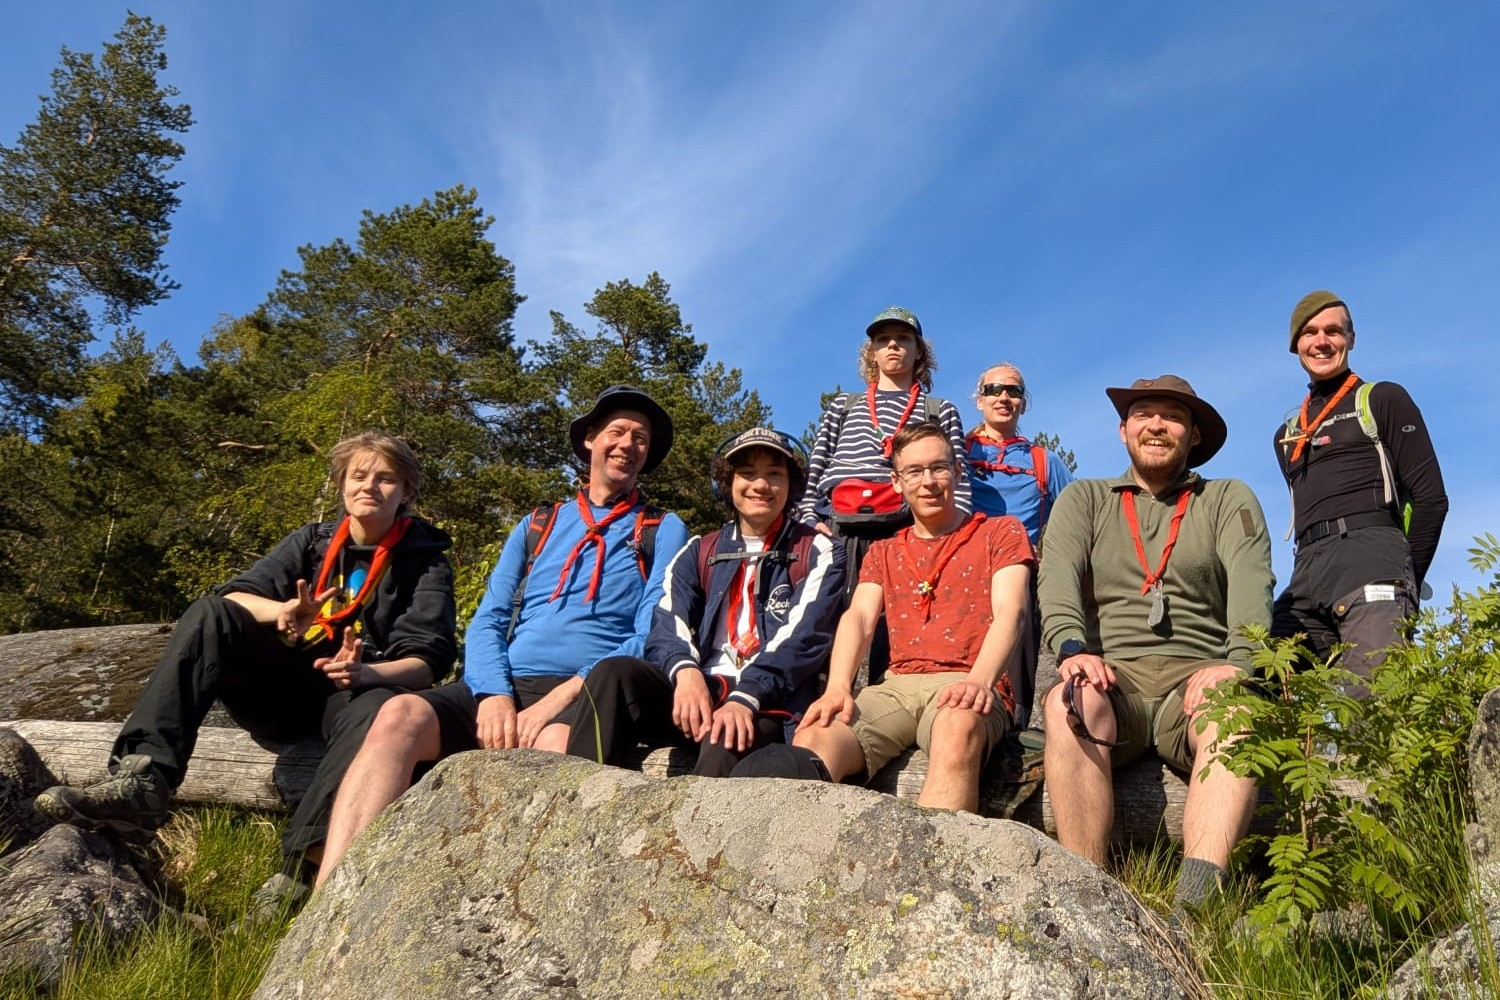
\includegraphics[width=\textwidth]{assets/liljaryhma.jpg}
\caption{\textit{Punaharmaa ja kahdeksas matkustaja} "=vartion ryhmäkuva 
Viikinrannan kalliolla, kun takana on jo noin 47 kilometriä.}
\end{figure}

\noindent\textit{Keväällä käveltiin punainen, viidenkymmenen kilometrin 
nahkalilja ja harmaa, kuudenkymmenen kilometrin nahkalilja. Liljaan kuuluu aina 
vartion kirjoittama raportti vaelluksesta. Raportti kirjoitetaan sekä vartiota 
itseään varten, jotta se voi pohtia ja mietiskellä yhteistä suoritustaan, 
että nahkaliljan myöntävää partiojohtajaa varten, jotta hän voi 
suorituksen tarkistaa; onhan se hauskaa palata ajassa taaksepäin ja lukea 
myöhemmin ajatuksista ja kommelluksista nahkaliljavaelluksilla! Tässä 
jutussa pääset lukemaan vartioiden yhdistelmäraportin.}

\begin{multicols}{2}
\noindent Ahti blaa blaa blaa

{\smallskip\noindent\centering ***\par\smallskip}

Neljä rusakkoa, Alden, Elias, Janne ja Toivo, nahkaliljavartio 
\textit{Punainen ja neljäs matkustaja}, starttasi punaisen nahkaliljan, 
viidenkymmenen kilometrin vuorokausivaelluksen Mikaelinkirkolta suunnitellusti 
\textbf{kello 8.00}. Yön aikana oli satanut kolmisen milliä vettä ja tiet 
olivat märkiä, mutta sääennusteessa lauantaipäivästä povattiin varsin 
aurinkoista. Lähtöön saapui viimeisenä Toivo, joka saikin kunnian toimia 
kartanlukijana ensimmäisen viiden kilometrin etapin ajan.

Huolella suunniteltu kymmenen kilometrin kierros Kontulassa, Myllypurossa, 
Latokartanossa ja Kivikossa suuntasi ensin etelään kohti Kontulan 
kelkkapuistoa. Kävellessä keskusteltiin nahkaliljaan mukaan otetuista 
eväistä ja juotavista, kuinka aikaisemmista liljoista oltiin opittu ja nyt 
paremmin varauduttu. Öinen sade oli houkutellut etanat, kotilot ja lierot 
kävelyteille ja vartio olikin valmis uudelleennimeämään Hietajärvenpolun 
Etanapoluksi matkalla kohti Mustapuronpuistoa. (Toim. huom. tässä vaiheessa 
ei vielä tiedetty, että myöhemmin reitille osuisi oikea Etanapolku 
Yliskylässä.) Suurin osa kierroksesta oli hiekkatietä, minkä vuoksi 
erityisesti kotiloita jouduttiin väistelemään melkein koko aamu. 

Lähestyttäessä Myllypuroa vartion keskustelu oli rönsyillyt jo opettajiin 
ja heidän tunnetuksi tulleisiin lausahduksiin ja pian kavuttiinkin 
Alakivenpuiston kuntoportaita ylös entiselle jätemäelle ottamaan punaisen 
liljan suorittajista ryhmäkuva. Toivo seurasi reittiä ansiokkaasti, vaikka 
oikaisuvaihtoehto Myllytaipaleelle olikin houkutteleva: ''Hei, shortcut!''

Aikaisempien nahkaliljojen ja harjoitusmarssin muistelot siivittivät 
vaellusta. Ensimmäinen etappi oli taitettu \textbf{kello 9.03} ja vartio 
pysähtyi tauolle Hallainvuoren juurelle. Tauko päätettiin pitää lyhyenä, 
jotta ennätettäisiin takaisin kirkolle kymmeneksi. Kartta vaihtui Aldenille 
ja reitin suunta kääntyi pohjoiseen. Luonnonsuojelualueen reunalla mietittiin 
hauskoja paikannimiä -- mainittiinpa ainakin Ii, Yksipuinen ja Pöljä. 

Viikin puistosilta palautti mieleen kevään 2024 nahkaliljan, jossa osa 
suorittajista oli henkisesti romahtanut sillan päässä. Tällä kertaa silta 
ei tuottanut yhdellekään vartion jäsenelle ongelmia, askel oli kevyt ja 
Alden tokaisi: ''I'm feeling really happy.''

Paukkulanpuistoon saavuttaessa arvuuteltiin, josko vartio törmäisi 
aikaisemmin kävelemään lähteneisiin harmaan nahkaliljan suorittajiin, 
\textit{Harmaa}"-vartioon. \textit{Punainen ja neljäs matkustaja} osoittautui 
olevan kuitenkin yli kymmenen minuuttia \textit{Harmaata} edellä, joten 
pysähtymättä jatkettiin kohti Kivikon ulkoilupuistoa. Aivan sattumalta 
vartiota tervehti neljä rusakkoa lumilautailurinteelle vievässä 
ylämäessä. Ehkä nekin olivat lauantaikävelyllä!

Reitin kaartaessa takaisin kirkolle päin puheenaihe oli vaihtunut Hawkingin 
säteilyyn, jota Toivolla oli haasteita kuvailla. Säästämme lukijoilta 
säteilyn varsinaisen määritelmän, mutta kukin voi halutessaan sen verkosta 
tarkistaa. Juuri parahiksi aurinko alkoi pilkistää pilvien välistä vartion 
saapuessa kirkolle \textbf{kello 10.06}. Kirkolla pidettiin vajaan tunnin 
tauko, jonka jälkeen yhdistelmävartio \textit{Punaharmaa ja kahdeksas 
matkustaja} jatkoi matkaa yhteiselle neljänkymmenen kilometrin kierrokselle. 

{\smallskip\noindent\centering ***\par\smallskip}

Ahti blaa blaa blaa

Punaisen ja harmaan nahkaliljojen reittien pituuksiksi tuli tarkistusmittausten 
jälkeen 49,4 ja 59,5 kilometriä, mitkä tarkoittivat noin 3,6 ja 3,8 
kilometrin tuntivauhteja. Muut siirtymät ja taukoliikkumiset mukaan lukien 
kaikki suorittajat saavuttivat liljoissa vaaditut matkat. 

Ilmatieteen laitoksen Kumpulan havaintoasemalla merkittiin vaelluspäivän 
sääksi selkeästä pilviseen, lämpötila 7--14 astetta, lounastuulta, joka 
kääntyi itätuuleksi, 1--4 metriä sekunnissa ja ilmankosteus 53--98 
prosenttia -- mitä erinomaisin nahkaliljakeli!
\end{multicols}

\vfill

\noindent\null\hfill Kuvat: Tanguy\\
\noindent\null\hfill Teksti: Ahti ja Janne
